\documentclass[spanish, aspectratio=169]{beamer}
\usetikzlibrary{shapes.geometric}
\usepackage[es-tabla]{babel}
\usepackage{parskip}
\usepackage[capitalise, noabbrev]{cleveref}
\crefname{table}{\spanishtablename}{\spanishtablename}



\title{
	\textbf{
		Desarrollo de un modelo fundacional estocástico basado en procesos Gaussianos para la clasificación de bioseñales EEG en el diagnóstico asistido del TDAH.
	}
	}
\author{
	Julián David Pastrana Cortés, M.Sc.
	}


\date{}

\begin{document}
	
	
\frame{\titlepage}

\begin{frame}{Motivation}
	\vspace{-0.5cm}
	\begin{block}{}
		Mental disorders affect cognition, behavior, and emotions of millions of people worldwide. Around 350 million individuals suffer from a mental disorder \cite{Dehghan-Bonari2023}.
	\end{block}
	
	\begin{columns}
		\small
		\vspace{-0.2cm}
		\column{0.33\textwidth}
		\centering
		
\includegraphics[width=0.5\textwidth]{figures/OppositionalDefiantDisorder.png}
		
		\vspace{0.5em}
		\textbf{Oppositional Defiant Disorder}
		
		\column{0.33\textwidth}
		\centering
		
\includegraphics[width=0.5\textwidth]{figures/BipolarDisorder.png}
		
		\vspace{0.5em}
		\textbf{Bipolar Disorder}
		
		\column{0.33\textwidth}
		\centering
		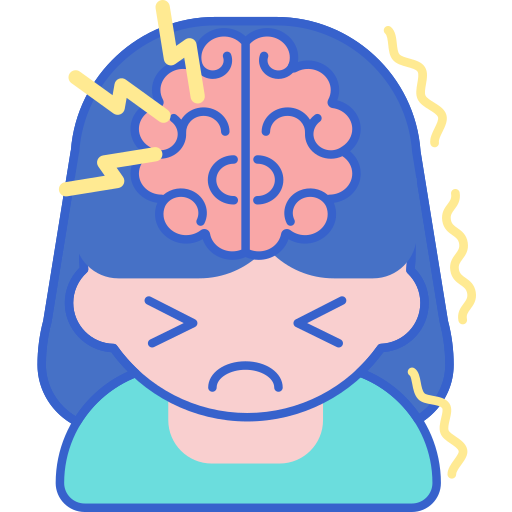
\includegraphics[width=0.5\textwidth]{figures/ADHD.png}
		
%		\vspace{0.5em}
		\textbf{Attention Deficit Hyperactivity Disorder}
	\end{columns}
%	\vspace{-0.5cm}
	\pause
	\begin{block}{Challenges:}
		lengthy follow-up, subjective interpretations, inefficient criteria, and limited access to clinical care.
	\end{block}
	
\end{frame}

\begin{frame}{Problem Statement and Research Question}
	
\renewcommand{\arraystretch}{1.5} 

\begin{table}[htbp]
	\centering
	\footnotesize
	\begin{tabular}{>{\raggedright\arraybackslash}p{3.1cm} >{\centering\arraybackslash}p{2cm} >{\centering\arraybackslash}p{2cm} >{\centering\arraybackslash}p{2cm} >{\centering\arraybackslash}p{2cm}}
		\toprule
		\diagbox{\textbf{Model}}{\textbf{Challenge}} & \textbf{Complex Patterns} & \textbf{High Labeled Data Volume} & \textbf{Stochasticity} & \textbf{Data Shift} \\
		\midrule
		Machine Learning \cite{Salari2023} & \textcolor{purple}{\ding{55}} & \textcolor{teal}{\ding{51}} & \textcolor{teal}{\ding{51}} & \textcolor{purple}{\ding{55}} \\[1mm]
		Deep Learning  \cite{LOHANI2023111689}    & \textcolor{teal}{\ding{51}}    & \textcolor{purple}{\ding{55}} & \textcolor{teal}{\ding{51}} & \textcolor{teal}{\ding{51}} \\[1mm]
		Foundation \cite{Sibley21042021}                   & \textcolor{teal}{\ding{51}}    & \textcolor{teal}{\ding{51}}    & \textcolor{purple}{\ding{55}} & \textcolor{teal}{\ding{51}} \\
		\bottomrule
	\end{tabular}

\end{table}

\pause	
	
	\begin{block}{Research Question}
		\footnotesize
		How to develop a stochastic foundational model for inference from biological signals that integrates Gaussian processes to support clinical practice through EEG signal analysis, considering the variability and inconsistencies present in the datasets?
	\end{block}	
\end{frame}



\begin{frame}{Objectives}
%	\vspace{-0.3cm}
	\begin{block}{General Objective}
		\small
		Develop a stochastic learning methodology related to EEG recordings based on a foundational model that integrates labeled and unlabeled databases using self-learning and fine-tuning techniques.
	\end{block}
	
	\vspace{-0.1cm}
	\begin{block}{Specific Objectives}
		\small
		\begin{enumerate}
			\item Develop a foundational model for the classification of biological signals related to EEG recordings, leveraging \textcolor{MyAccent}{unlabeled data} during the self-learning phase and labeled data for fine-tuning.
			\item Implement a \textcolor{MyAccent}{stochastic prediction} tool based on Gaussian processes to model uncertainty in the foundational model's predictions.
			\item Design a strategy to \textcolor{MyAccent}{manage variability and inconsistency} in EEG recording datasets, enabling the effective integration of databases with diverse standards.
		\end{enumerate}
	\end{block}
\end{frame}




\section{The Dataset}

\begin{frame}{Problem Setting}
	\begin{block}{}
		We define the multimodal input space as the Cartesian product of $P$ modality-specific input spaces:
		\[
		\mathcal{X} = \prod_{p=1}^{P} \mathcal{X}^{(p)},
		\]
		where each modality $\mathcal{X}^{(p)}$ may represent data from distinct sources.
	\end{block}
	
\end{frame}



\begin{frame}{Toadstool 2 Dataset}
\begin{block}{}
The dataset consists of video, sensor, and demographic data collected from 10 participants playing a Super Mario Bros.
\end{block}

\vspace{-0.5em}

		\begin{columns}[T] % Top alignment
		\begin{column}{0.5\textwidth}
			\begin{center}
\begin{tikzpicture}
	\begin{axis}[
		width=\textwidth,
		height=4cm,
		ybar,
		bar width=12pt,
		axis x line=bottom,
		axis y line=left,
		ylabel={\% of Samples},
		symbolic x coords={0,1,2,3,4,5,6},
		xtick=data,
%		xticklabel style={rotate=0,anchor=east},
		enlarge x limits=0.1,
		ymin=0, ymax=60
		]
		\addplot+[fill=blue!60] coordinates {
			(0,10) (1,10) (2,10) (3,10) (4,5) (5,4) (6,51)
		};
	\end{axis}
\end{tikzpicture}

  \begin{columns}[t]
	\column{0.33\textwidth}
	\centering\footnotesize
	\begin{tabular}{r l}
		0 & Anger   \\
		1 & Disgust \\
		2 & Fear    
	\end{tabular}
	
	\column{0.33\textwidth}
	\centering\footnotesize
	\begin{tabular}{r l}
		3 & Happy     \\
		4 & Sad       \\
		5 & Surprised 
	\end{tabular}
	
	\column[c]{0.33\textwidth}
	\centering\footnotesize
	\begin{tabular}{r l}
		6 & Neutral\\
		  &  \\
		  &
	\end{tabular}
\end{columns}



			\end{center}
			
		\end{column}
		\begin{column}{0.5\textwidth}
		\centering
		\small
		\begin{tabular}{lcc}
		\toprule
		\textbf{Signal} & \textbf{Rate (Hz)} & \textbf{Channels} \\
		\midrule
		BVP  & 64 & 1      \\
		ACC  & 32 & 3 		\\
		EDA  & 4  & 1      \\
		HR   & 1  & 1      \\
		\bottomrule
		\end{tabular}
		
		\begin{block}{}
			20 970 sensor‐only samples (4 s windows)
		\end{block}

		\end{column}
		
	\end{columns}
\end{frame}


\begin{frame}[t]{Problem Setting}
	\begin{block}{}
		Let $\{(\boldsymbol{x}^{(i)},\,y^{(i)})\}_{i=1}^N$ be the training dataset, where 
		$\boldsymbol{x}^{(i)}\in\mathcal{X}$ and $y^{(i)}\in\{0,1,\dots,6\}$.  
		Here $\mathcal{X}$ is the space of vector sequences of length $T=256$:
		\[
		\boldsymbol{x}^{(i)}
		= \bigl[\boldsymbol{x}^{(i)}_{1}, \dots, \boldsymbol{x}^{(i)}_{t}, \dots,\boldsymbol{x}^{(i)}_{T}\bigr].
		\]
		Each vector $\boldsymbol{x}^{(i)}_{t}$ has $p=6$ elements by channels,
		denoted $x^{(i)}_{t,j}\in\mathbb{R}$ or be a missing value $\hat{x}^{(i)}_{t,j}$.
	\end{block}
	
\begin{center}
	\begin{tikzpicture}[x=1.2cm,y=1.2cm]
		\foreach \i in {0,...,4} {
			\fill[MyAccent!20] (\i,0) rectangle ++(1,1);
			\node[text=white, font=\footnotesize] at (\i+0.5,0.5) {t=\i};
		}
	\end{tikzpicture}
\end{center}
\end{frame}




\section[\empty]{Objective 1: Foundation Model}

\begin{frame}[fragile]{Objective 1: Foundation Model}
	
	\begin{block}{}
		We aims to train a general model using large amounts of data and tasks that can be fine-tuned easily in different downstream applications.
	\end{block}
	\centering
	\resizebox{\textwidth}{!}{
		\begin{tikzpicture}[font=\sffamily, >=stealth, node distance=3cm, thick]
			
			% Left Square (Training)
			\node[rectangle, draw=MyAccent, fill=MyLightGray, rounded corners, align=left, text=MyDarkBlue] (training) {
				\textbf{Data}\\[5pt]
				- Text\\
				- Images\\
				- Sensors\\
				- Speech
			};
			
			% Foundation Model (center)
			\node[rectangle, draw=MyAccent, fill=MyAccent!20, rounded corners, minimum width=3.5cm, minimum height=2cm, right=of training, text=MyDarkBlue] (foundation) {
				\textbf{Foundation Model}
			};
			
			% Right Square (Tasks)
			\node[rectangle, draw=MyAccent, fill=MyLightGray, rounded corners, align=left, right=of foundation, text=MyDarkBlue] (tasks) {
				\textbf{Task}\\[5pt]
				- Object Recognition\\
				- Text Generation\\
				- Sentiment Analysis\\
				- Image Captioning
			};
			
			% Arrows
			\draw[->, MyDarkBlue] (training.east) -- node[above, text=MyDarkBlue]{Pre-Training} (foundation.west);
			\draw[->, MyDarkBlue] (foundation.east) -- node[above, text=MyDarkBlue]{Fine-Tuning} (tasks.west);
			
		\end{tikzpicture}
	}
\end{frame}


\begin{frame}[fragile]{Architecture}
	\begin{block}{}
		We can leverage large amounts of unlabeled data to learn hidden‐state representations without committing to any specific downstream task.
	\end{block}
	
	\resizebox{\textwidth}{!}{
		\tikzset{trapezium stretches=true}
		\centering
		\begin{tikzpicture}[font=\sffamily, >=stealth, node distance=8mm]
			% Latent variable (z)
			\node[rectangle, fill=MyAccent, text=white, font=\sffamily\large, minimum height=3cm, text width=3cm, align=center] (z) {Latent\\ Representation ($\boldsymbol{h}$)};
			
			% Encoder trapezoid
			\node[trapezium, fill=MyAccent!20, minimum width=4cm, minimum height=4cm,
			trapezium left angle=86, trapezium right angle=86, shape border rotate=270,
			anchor=east, left=5mm of z, font=\sffamily\large, text=MyDarkBlue] (enc) {Encoder};
			
			% Decoder trapezoid
			\node[trapezium, fill=MyAccent!20, minimum width=4cm, minimum height=4cm,
			trapezium left angle=86, trapezium right angle=86, shape border rotate=90,
			anchor=west, right=5mm of z, font=\sffamily\large, text=MyDarkBlue] (dec) {Decoder};
			
		
			% Arrows and labels
			\draw[<-, MyDarkBlue, thick] (enc.west) -- ++(-1.5,0) node[left, align=right, text=MyDarkBlue] {Input};
			\draw[->, MyDarkBlue, thick] (dec.east) -- ++(1.5,0) node[right, align=left, text=MyDarkBlue] {Reconstruction};
%			\draw[->, MyAccent, thick] (z.south) -- (gp.north);
%			\draw[->, MyDarkBlue, thick] (gp.east) -- ++(1.5,0) node[right, align=left, text=MyDarkBlue] {Predictive Distribution\\(Inference)};
		\end{tikzpicture}
	}
\end{frame}



\section{Objective 2}
\begin{frame}{Objetive 2: Gaussian Process}
		\centering
		\begin{tikzpicture}
			\begin{groupplot}[
				group style={
					group name=my plots,
					group size=2 by 1,
					horizontal sep=1cm,
				},
				width=5cm,
				height=4cm,
				scale only axis,
				axis lines=left,
				ymin=0, ymax=1,
				xmin=0, xmax=5.5,
				xlabel style={text=MyDarkBlue},
				title style={text=MyDarkBlue},
				]
				% Left subplot: Point Estimate Prediction
				\nextgroupplot[
				title={Point Estimation},
				xticklabel=\empty,
				yticklabel=\empty,
				]
				\addplot+[smooth, thick, color=MyAccent!30, mark=*,
				mark options={fill=MyAccent, draw=MyAccent}
				] coordinates {(0,0.2) (1,0.3) (2,0.5) (3,0.7) (4,0.8)};
				\addplot[only marks, mark=*, MyDarkBlue] coordinates {(5,0.85)};
				
				% Right subplot: Distribution Estimation with Error Bars
				\nextgroupplot[
				title={Distribution Estimation},
				xticklabel=\empty,
				yticklabel=\empty,
				]
				\addplot+[smooth, thick, color=MyAccent!30, mark=*,
				mark options={fill=MyAccent, draw=MyAccent}
				] coordinates {(0,0.2) (1,0.3) (2,0.5) (3,0.7) (4,0.8)};
				
				% Predictive distribution at time=5
				\addplot[name path=right, domain=0.65:1.05, variable=\y, samples=100, draw=none]
				({5 + 0.2*exp(-((\y-0.85)^2)/(2*0.004))}, {\y});
				
				\addplot[name path=left, domain=0.65:1.05, variable=\y, samples=100, draw=none]
				({5 - 0.2*exp(-((\y-0.85)^2)/(2*0.004))}, {\y});
				
				\addplot[fill=MyAccent!50, fill opacity=0.4, draw=none]
				fill between[of=right and left];
				
				\addplot[only marks, mark=*, MyDarkBlue] coordinates {(5,0.85)};
				
			\end{groupplot}
		\end{tikzpicture}
		
		\begin{block}{}
			Sometimes, a single point prediction is not enough. How confident is the model in its prediction?
		\end{block}
\end{frame}


\begin{frame}[fragile]{Architecture}
	\resizebox{\textwidth}{!}{
		\tikzset{trapezium stretches=true}
		\centering
		\begin{tikzpicture}[font=\sffamily, >=stealth, node distance=8mm]
			% Latent variable (z)
			\node[rectangle, fill=MyAccent, text=white, font=\sffamily\large, minimum height=3cm, text width=3cm, align=center] (z) {Latent\\ Representation ($\boldsymbol{h}$)};
			
			% Encoder trapezoid
			\node[trapezium, fill=MyAccent!20, minimum width=4cm, minimum height=4cm,
			trapezium left angle=86, trapezium right angle=86, shape border rotate=270,
			anchor=east, left=5mm of z, font=\sffamily\large, text=MyDarkBlue] (enc) {Encoder};
			
			% Decoder trapezoid
			\node[trapezium, fill=MyAccent!20, minimum width=4cm, minimum height=4cm,
			trapezium left angle=86, trapezium right angle=86, shape border rotate=90,
			anchor=west, right=5mm of z, font=\sffamily\large, text=MyDarkBlue] (dec) {Decoder};
			
			% Gaussian Process circle
			\node[circle, fill=MyAccent!20, text=MyDarkBlue, font=\sffamily\small,
			below=2cm of z, minimum size=2cm, align=center] (gp) {Gaussian\\Process};
			
			% Arrows and labels
			\draw[<-, MyDarkBlue, thick] (enc.west) -- ++(-1.5,0) node[left, align=right, text=MyDarkBlue] {Input};
			\draw[->, MyDarkBlue, thick] (dec.east) -- ++(1.5,0) node[right, align=left, text=MyDarkBlue] {Reconstruction};
			\draw[->, MyAccent, thick] (z.south) -- (gp.north);
			\draw[->, MyDarkBlue, thick] (gp.east) -- ++(1.5,0) node[right, align=left, text=MyDarkBlue] {Predictive Distribution\\(Inference)};
		\end{tikzpicture}
	}
\end{frame}

\begin{frame}{Chained Correlated GP }
	\centering
	\begin{tikzpicture}[x=4.5cm,y=1.5cm]
		% \message{^^JNeural network activation}
		\def\NI{4} % number of nodes in input layer
		\def\NM{4} % number of nodes in middle layer  
		\def\NO{2} % number of nodes in output layer
		\def\yshift{0.0} % shift last node for dots
		
		% INPUT LAYER
		\foreach \i [evaluate={\c=int(\i==\NI); \y=\NI/2-\i-\c*\yshift; \index=(\i<\NI?int(\i):"Q");}]
		in {1,...,\NI}{ % loop over nodes
			\node[node in,outer sep=0.6] (NI-\i) at (0,\y) {$u_{\index}$};
		}
		
		% MIDDLE LAYER
		
		% MIDDLE LAYER with specific labels
		\node[node hidden] (NM-1) at (1,\NM/2-1) {$f_{1, J_1}$};
		\node[node hidden] (NM-2) at (1,\NM/2-2) {$f_{2, J_1}$};
		\node[node hidden] (NM-3) at (1,\NM/2-3) {$f_{1, J_D}$};
		\node[node hidden] (NM-4) at (1,\NM/2-4) {$f_{D, J_D}$};
		
		\foreach \i [evaluate={\c=int(\i==\NM); \y=\NM/2-\i-\c*\yshift; \index=(\i<\NM?int(\i):"D");}]
		in {\NM,...,1}{ % loop over nodes
			\ifnum\i=1 % highlighted node
			\foreach \j [evaluate={\index=(\j<\NI?int(\j):"Q");}] in {1,...,\NI}{ % loop over nodes in previous layer
				\draw[connect,white,line width=1.2] (NI-\j) -- (NM-\i);
				\draw[connect] (NI-\j) -- (NM-\i)
				node[pos=0.50] {\contour{white}{$a_{1, 1,\index}$}};
			}
			\else % other light-colored nodes
			\foreach \j in {1,...,\NI}{ % loop over nodes in previous layer
				\draw[connect,white,line width=1.2] (NI-\j) -- (NM-\i);
				\draw[connect,myblue!20] (NI-\j) -- (NM-\i);i
			}
			\fi
		}
		
		
		% OUTPUT LAYER
		\foreach \i [evaluate={\c=int(\i==\NO); \y=\NO/2-\i-\c*\yshift; \index=(\i<\NO?int(\i):"D");}]
		in {\NO,...,1}{ % loop over nodes
			\ifnum\i=1 % highlighted node
			\node[node out]
			(NO-\i) at (2,\y) {$y_{\index}$};
			\foreach \j [evaluate={\index=(\j<3?int(\j):"D");}] in {1,2}{ % loop over nodes 1 and 2 in middle layer
				\draw[connect,white,line width=1.2] (NM-\j) -- (NO-\i);
				\draw[connect, myred] (NM-\j) -- (NO-\i)
				node[pos=0.50] {\contour{white}{$g_{\index,J_{1}}(\cdot)$}};
			}
			\else % other light-colored nodes
			\node[node out]
			(NO-\i) at (2,\y) {$y_{\index}$};
			\foreach \j in {3,4}{ % loop over nodes 3 and 4 in middle layer
				\draw[connect,white,line width=1.2] (NM-\j) -- (NO-\i);
				\draw[connect,myred!20] (NM-\j) -- (NO-\i);
			}
			\fi
		}
		
		
		% DOTS
		\path (NI-\NI) --++ (0,1+\yshift) node[midway,scale=1.2] {$\vdots$};
		\path (NM-\NM) --++ (0,3+\yshift) node[midway,scale=1.2] {$\vdots$};
		\path (NM-\NM) --++ (0,1+\yshift) node[midway,scale=1.2] {$\vdots$};
		\path (NO-\NO) --++ (0,1+\yshift) node[midway,scale=1.2] {$\vdots$};
		
	\end{tikzpicture}
	\scriptsize
	\begin{columns}[T] % Top alignment
		\begin{column}{0.33\textwidth}
			\centering	
			\textcolor{mygreen}{
				\textbf{Independent Process}
				\vspace{-1.3em}
							\begin{equation*}
									u_{q}(\mathbf{h}) \sim \mathcal{GP}(0, k_{q}(\mathbf{h}, \mathbf{h}'))
								\end{equation*}
			}
		\end{column}
		
		\begin{column}{0.33\textwidth}
			\centering
			\textcolor{myblue}{
				\textbf{Latent Process}
				\vspace{-1.3em}
							\begin{equation*}
									f_{d,j}(\mathbf{h}) = \sum_{q=1}^Q a_{d,j,q} u_{q}(\mathbf{h})
								\end{equation*}
			}
		\end{column}
		
		\begin{column}{0.33\textwidth}
			\centering
			\textcolor{myred}{
				\textbf{Likelihood}
				\vspace{-1.3em}
							\begin{equation*}
									\mathbf{y} \mid \mathbf{f} \sim \prod_{d=1}^D p(\theta_{d, 1}, \cdots, \theta_{d, J_d})
								\end{equation*}
							\vspace{-1.5em}
							\begin{equation*}
									\theta_{d, j} = g_{d, j}(f_{d, j})
								\end{equation*}
			}
		\end{column}
		
	\end{columns}
\end{frame}
\section[\empty]{Objective 3: Long Short-Term Memory (LSTM) Architecture}

\begin{frame}{Objective 3: Long Short-Term Memory (LSTM) Architecture}
\begin{columns}[t]
\begin{column}{0.65\textwidth}


\begin{tikzpicture}[
	% GLOBAL CFG
	font=\sf \scriptsize,
	>=LaTeX,
	% Styles
	cell/.style={% For the main box
		rectangle, 
		rounded corners=5mm, 
		draw,
		very thick,
	},
	operator/.style={%For operators like +  and  x
		circle,
		draw,
		inner sep=-0.5pt,
		minimum height =.2cm,
	},
	function/.style={%For functions
		ellipse,
		draw,
		inner sep=1pt
	},
	ct/.style={% For external inputs and outputs
		circle,
		draw,
		line width = .75pt,
		minimum width=1cm,
		inner sep=1pt,
	},
	gt/.style={% For internal inputs
		rectangle,
		draw,
		minimum width=4mm,
		minimum height=3mm,
		inner sep=1pt
	},
	mylabel/.style={% something new that I have learned
		font=\scriptsize\sffamily
	},
	ArrowC1/.style={% Arrows with rounded corners
		rounded corners=.25cm,
		thick,
	},
	ArrowC2/.style={% Arrows with big rounded corners
		rounded corners=.5cm,
		thick,
	},
	]
	
	%Start drawing the thing...    
	% Draw the cell: 
	\node [cell, minimum height =4cm, minimum width=6cm] at (0,0){} ;
	
	% Draw inputs named ibox#
	\node [gt] (ibox1) at (-2,-0.75) {$\sigma$};
	\node [gt] (ibox2) at (-1.5,-0.75) {$\sigma$};
	\node [gt, minimum width=1cm] (ibox3) at (-0.5,-0.75) {Tanh};
	\node [gt] (ibox4) at (0.5,-0.75) {$\sigma$};
	
	% Draw opérators   named mux# , add# and func#
	\node [operator] (mux1) at (-2,1.5) {$\times$};
	\node [operator] (add1) at (-0.5,1.5) {+};
	\node [operator] (mux2) at (-0.5,0) {$\times$};
	\node [operator] (mux3) at (1.5,0) {$\times$};
	\node [function] (func1) at (1.5,0.75) {Tanh};
	
	% Draw External inputs? named as basis c,h,x
	\node[ct, label={[mylabel]Cell}] (c) at (-4,1.5) {$\boldsymbol{c}_{t-1}$};
	\node[ct, label={[mylabel]Hidden}] (h) at (-4,-1.5) {$\boldsymbol{h}_{t-1}$};
	\node[ct, label={[mylabel]left:Input}] (x) at (-2.5,-3) {{$\boldsymbol{x}_{t}^{(i)}$}};
	
	% Draw External outputs? named as basis c2,h2,x2
	\node[ct, label={[mylabel]\empty}] (c2) at (4,1.5) {$\boldsymbol{c}_{t}$};
	\node[ct, label={[mylabel]\empty}] (h2) at (4,-1.5) {$\boldsymbol{h}_{t}$};
%	\node[ct, label={[mylabel]left:\empty}] (x2) at (2.5,3) {$\boldsymbol{h}_{t}$};
	
	% Start connecting all.
	%Intersections and displacements are used. 
	% Drawing arrows    
	\draw [ArrowC1] (c) -- (mux1) -- (add1) -- (c2);
	
	% Inputs
	\draw [ArrowC2] (h) -| (ibox4);
	\draw [ArrowC1] (h -| ibox1)++(-0.5,0) -| (ibox1); 
	\draw [ArrowC1] (h -| ibox2)++(-0.5,0) -| (ibox2);
	\draw [ArrowC1] (h -| ibox3)++(-0.5,0) -| (ibox3);
	\draw [ArrowC1] (x) -- (x |- h)-| (ibox3);
	
	% Internal
	\draw [->, ArrowC2] (ibox1) -- (mux1);
	\draw [->, ArrowC2] (ibox2) |- (mux2);
	\draw [->, ArrowC2] (ibox3) -- (mux2);
	\draw [->, ArrowC2] (ibox4) |- (mux3);
	\draw [->, ArrowC2] (mux2) -- (add1);
	\draw [->, ArrowC1] (add1 -| func1)++(-0.5,0) -| (func1);
	\draw [->, ArrowC2] (func1) -- (mux3);
	
	%Outputs
	\draw [-, ArrowC2] (mux3) |- (h2);
%	\draw (c2 -| x2) ++(0,-0.1) coordinate (i1);
	\draw [-, ArrowC2] (h2 -| x2)++(-0.5,0) -| (i1);
%	\draw [-, ArrowC2] (i1)++(0,0.2) -- (x2);
	
\end{tikzpicture}
\end{column}

    % equations column, also top‐aligned
\begin{column}[t]{0.45\textwidth}

	\small
	\begin{align*}
\boldsymbol{i}_t &= \sigma\bigl(\boldsymbol{W}_{ii}\,\boldsymbol{x}_t^{(i)} 
+ \boldsymbol{W}_{hi}\,\boldsymbol{h}_{t-1}
+ \boldsymbol{b}_i\bigr),\\
\boldsymbol{f}_t &= \sigma\bigl(\boldsymbol{W}_{if}\,\boldsymbol{x}_t^{(i)} 
+ \boldsymbol{W}_{hf}\,\boldsymbol{h}_{t-1}
+ \boldsymbol{b}_f\bigr),\\
\boldsymbol{g}_t &= \tanh\bigl(\boldsymbol{W}_{ig}\,\boldsymbol{x}_t^{(i)} 
+ \boldsymbol{W}_{hg}\,\boldsymbol{h}_{t-1}
+ \boldsymbol{b}_g\bigr),\\
\boldsymbol{o}_t &= \sigma\bigl(\boldsymbol{W}_{io}\,\boldsymbol{x}_t^{(i)} 
+ \boldsymbol{W}_{ho}\,\boldsymbol{h}_{t-1}
+ \boldsymbol{b}_o\bigr),\\
\boldsymbol{C}_t &= \boldsymbol{f}_t \odot \boldsymbol{C}_{t-1}
+ \boldsymbol{i}_t \odot \boldsymbol{g}_t,\\
\boldsymbol{h}_t &= \boldsymbol{o}_t \odot \tanh\bigl(\boldsymbol{C}_t\bigr).
	\end{align*}
	
\(\odot\) is the Hadamard product, and \(\sigma\) the sigmoid function.

	
\end{column}
\end{columns}


\end{frame}
	
\begin{frame}[t]{Missing‐Value Imputation}
	\begin{columns}[t]
		\begin{column}{0.55\textwidth}
			\begin{block}{}
				At each time step \(t\), missing channel entries in \(\boldsymbol{x}_t^{(i)}\) can be imputed sequentially from the hidden state via an affine map:
				\[
				\hat{x}_{t,j}^{(i)}
				= \boldsymbol{w}_j^{\mathsf T}\,\boldsymbol{h}_t + b_j,
				\quad j = 1,\dots,p.
				\]
			\end{block}

		\end{column}
		\begin{column}{0.45\textwidth}
			\[
			\begin{aligned}
				\{\boldsymbol{W}_{ii},\,\boldsymbol{W}_{if},\,\boldsymbol{W}_{ig},\,\boldsymbol{W}_{io}\}
				&\in \mathbb{R}^{H \times p},\\
				\{\boldsymbol{W}_{hi},\,\boldsymbol{W}_{hf},\,\boldsymbol{W}_{hg},\,\boldsymbol{W}_{ho}\}
				&\in \mathbb{R}^{H \times H},\\
				\{\boldsymbol{b}_{i},\,\boldsymbol{b}_{f},\,\boldsymbol{b}_{g},\,\boldsymbol{b}_{o}\}
				&\in \mathbb{R}^{H},\\
				\boldsymbol{w}_j &\in \mathbb{R}^{H},\\
				b_j &\in \mathbb{R},\\
				\boldsymbol{h}_t,\,\boldsymbol{C}_t &\in \mathbb{R}^{H}.
			\end{aligned}
			\]
			Here \(H\) denotes the dimensionality of the hidden state.
		\end{column}
	\end{columns}
\end{frame}

\begin{frame}[fragile]{Architecture}
	\resizebox{\textwidth}{!}{
		\tikzset{trapezium stretches=true}
		\centering
		\begin{tikzpicture}[font=\sffamily, >=stealth, node distance=8mm]
			% Latent variable (z)
			\node[rectangle, fill=MyAccent, text=white, font=\sffamily\large, minimum height=3cm, text width=3cm, align=center] (z) {Latent\\ Representation ($\boldsymbol{h}$)};
			
			% Encoder trapezoid
			\node[trapezium, fill=MyAccent!20, minimum width=4cm, minimum height=4cm,
			trapezium left angle=86, trapezium right angle=86, shape border rotate=270,
			anchor=east, left=5mm of z, font=\sffamily\large, text=MyDarkBlue] (enc) {Encoder (LSTM)};
			
			
			% Gaussian Process circle
			\node[circle, fill=MyAccent!20, text=MyDarkBlue, font=\sffamily\small,
			below=2cm of z, minimum size=2cm, align=center] (gp) {Gaussian\\Process};
			
			% Arrows and labels
			\draw[<-, MyDarkBlue, thick] (enc.west) -- ++(-1.5,0) node[left, align=right, text=MyDarkBlue] {Input};
			\draw[->, MyAccent, thick] (z.south) -- (gp.north);
			\draw[->, MyDarkBlue, thick] (gp.east) -- ++(1.5,0) node[right, align=left, text=MyDarkBlue] {Predictive Distribution\\(Inference)};
		\end{tikzpicture}
	}
\end{frame}
	
\bibliographystyle{apalike}
\bibliography{ref}
\end{document}
